\documentclass[]{article}
\usepackage{lmodern}
\usepackage{amssymb,amsmath}
\usepackage{ifxetex,ifluatex}
\usepackage{fixltx2e} % provides \textsubscript
\ifnum 0\ifxetex 1\fi\ifluatex 1\fi=0 % if pdftex
  \usepackage[T1]{fontenc}
  \usepackage[utf8]{inputenc}
\else % if luatex or xelatex
  \ifxetex
    \usepackage{mathspec}
  \else
    \usepackage{fontspec}
  \fi
  \defaultfontfeatures{Ligatures=TeX,Scale=MatchLowercase}
\fi
% use upquote if available, for straight quotes in verbatim environments
\IfFileExists{upquote.sty}{\usepackage{upquote}}{}
% use microtype if available
\IfFileExists{microtype.sty}{%
\usepackage{microtype}
\UseMicrotypeSet[protrusion]{basicmath} % disable protrusion for tt fonts
}{}
\usepackage[margin=1in]{geometry}
\usepackage{hyperref}
\hypersetup{unicode=true,
            pdftitle={Student Performance Analysis},
            pdfauthor={Zixin Zhang, Yenan Zhang},
            pdfborder={0 0 0},
            breaklinks=true}
\urlstyle{same}  % don't use monospace font for urls
\usepackage{longtable,booktabs}
\usepackage{graphicx,grffile}
\makeatletter
\def\maxwidth{\ifdim\Gin@nat@width>\linewidth\linewidth\else\Gin@nat@width\fi}
\def\maxheight{\ifdim\Gin@nat@height>\textheight\textheight\else\Gin@nat@height\fi}
\makeatother
% Scale images if necessary, so that they will not overflow the page
% margins by default, and it is still possible to overwrite the defaults
% using explicit options in \includegraphics[width, height, ...]{}
\setkeys{Gin}{width=\maxwidth,height=\maxheight,keepaspectratio}
\IfFileExists{parskip.sty}{%
\usepackage{parskip}
}{% else
\setlength{\parindent}{0pt}
\setlength{\parskip}{6pt plus 2pt minus 1pt}
}
\setlength{\emergencystretch}{3em}  % prevent overfull lines
\providecommand{\tightlist}{%
  \setlength{\itemsep}{0pt}\setlength{\parskip}{0pt}}
\setcounter{secnumdepth}{0}
% Redefines (sub)paragraphs to behave more like sections
\ifx\paragraph\undefined\else
\let\oldparagraph\paragraph
\renewcommand{\paragraph}[1]{\oldparagraph{#1}\mbox{}}
\fi
\ifx\subparagraph\undefined\else
\let\oldsubparagraph\subparagraph
\renewcommand{\subparagraph}[1]{\oldsubparagraph{#1}\mbox{}}
\fi

%%% Use protect on footnotes to avoid problems with footnotes in titles
\let\rmarkdownfootnote\footnote%
\def\footnote{\protect\rmarkdownfootnote}

%%% Change title format to be more compact
\usepackage{titling}

% Create subtitle command for use in maketitle
\newcommand{\subtitle}[1]{
  \posttitle{
    \begin{center}\large#1\end{center}
    }
}

\setlength{\droptitle}{-2em}

  \title{Student Performance Analysis}
    \pretitle{\vspace{\droptitle}\centering\huge}
  \posttitle{\par}
    \author{Zixin Zhang, Yenan Zhang}
    \preauthor{\centering\large\emph}
  \postauthor{\par}
    \date{}
    \predate{}\postdate{}
  

\begin{document}
\maketitle

\subsection{Introduction}\label{introduction}

It's common to see that many high school students now are in romantic
relationships. However, some parents think that having romantic
relationship will influence teenagers' academic performances. In this
project, we are interested in conducting research on an exploratory
question - \textbf{Does romantic relationship influence student's
academic performance?}.

We choose the dataset
\href{https://archive.ics.uci.edu/ml/datasets/Student+Performance}{Student
Performance Data Set} from UCL Machine Learning Repository. The dataset
have 30 attribute information and three academic grades of students in
math course and Portuguese language course. In this analysis, we will
use the dataset of students in math course. Based on our question, We
are only focusing on these two variables for our analysis: \texttt{G3} -
final grade (numeric: from 0 to 20, output target) and \texttt{romantic}
- with a romantic relationship (binary: yes or no).

\emph{Table 1. Student Performance Dataset}

\begin{longtable}[]{@{}rllrlllrrllllrrrllllllllrrrrrrrrrr@{}}
\toprule
X & school & sex & age & address & famsize & Pstatus & Medu & Fedu &
Mjob & Fjob & reason & guardian & traveltime & studytime & failures &
schoolsup & famsup & paid & activities & nursery & higher & internet &
romantic & famrel & freetime & goout & Dalc & Walc & health & absences &
G1 & G2 & G3\tabularnewline
\midrule
\endhead
1 & GP & F & 18 & U & GT3 & A & 4 & 4 & at\_home & teacher & course &
mother & 2 & 2 & 0 & yes & no & no & no & yes & yes & no & no & 4 & 3 &
4 & 1 & 1 & 3 & 6 & 5 & 6 & 6\tabularnewline
2 & GP & F & 17 & U & GT3 & T & 1 & 1 & at\_home & other & course &
father & 1 & 2 & 0 & no & yes & no & no & no & yes & yes & no & 5 & 3 &
3 & 1 & 1 & 3 & 4 & 5 & 5 & 6\tabularnewline
3 & GP & F & 15 & U & LE3 & T & 1 & 1 & at\_home & other & other &
mother & 1 & 2 & 3 & yes & no & yes & no & yes & yes & yes & no & 4 & 3
& 2 & 2 & 3 & 3 & 10 & 7 & 8 & 10\tabularnewline
4 & GP & F & 15 & U & GT3 & T & 4 & 2 & health & services & home &
mother & 1 & 3 & 0 & no & yes & yes & yes & yes & yes & yes & yes & 3 &
2 & 2 & 1 & 1 & 5 & 2 & 15 & 14 & 15\tabularnewline
5 & GP & F & 16 & U & GT3 & T & 3 & 3 & other & other & home & father &
1 & 2 & 0 & no & yes & yes & no & yes & yes & no & no & 4 & 3 & 2 & 1 &
2 & 5 & 4 & 6 & 10 & 10\tabularnewline
6 & GP & M & 16 & U & LE3 & T & 4 & 3 & services & other & reputation &
mother & 1 & 2 & 0 & no & yes & yes & yes & yes & yes & yes & no & 5 & 4
& 2 & 1 & 2 & 5 & 10 & 15 & 15 & 15\tabularnewline
\bottomrule
\end{longtable}

\subsection{Visualization}\label{visualization}

In order to better visualize our dataset, we choose the boxplot.

\emph{Figure 1. five numbers summary of the variable G3 facetted by
romantic}

\begin{figure}

{\centering 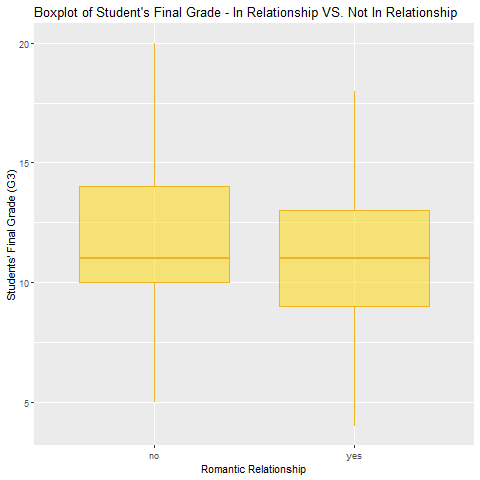
\includegraphics[width=6.67in]{../results/boxplot} 

}

\caption{Figure 1: Mean and spread for final grades}\label{fig:unnamed-chunk-3}
\end{figure}

The boxplot tells us five number summary of \texttt{G3} among the two
groups of students, with relationship and without relationship. The two
groups of student have similar mean of the final grade, but we found
that both the 25th percentile and 75th percentile of the group
\textbf{no} are higher than that of the group \textbf{yes}. The maximum
grade is in the group \textbf{no}, and the minimum grade is in the group
\textbf{yes}.

\subsection{Data summary}\label{data-summary}

In this part, we create a table which have statistical summary for in
relationship and single groups of students. We will report the mean of
final grade, sample size, 95\% confidence interval of each group. We
also visualize our data by a violin plot and jitter plot for the
G3(final grade) and facetted on relationship status.

\emph{Table 2. Statistical Summary of the Data}

\begin{longtable}[]{@{}rrrlrr@{}}
\toprule
X & lower & upper & romantic & mean & n\tabularnewline
\midrule
\endhead
1 & 11.20398 & 12.07347 & no & 11.63265 & 245\tabularnewline
2 & 10.76786 & 11.83058 & yes & 11.28571 & 112\tabularnewline
\bottomrule
\end{longtable}

\emph{Figure 2. Mean final grade for in-relationship and single groups
of students. Error bars represent 95\% confidence intervals generated by
boostrapping.}

\textbackslash{}begin\{figure\}

\{\centering 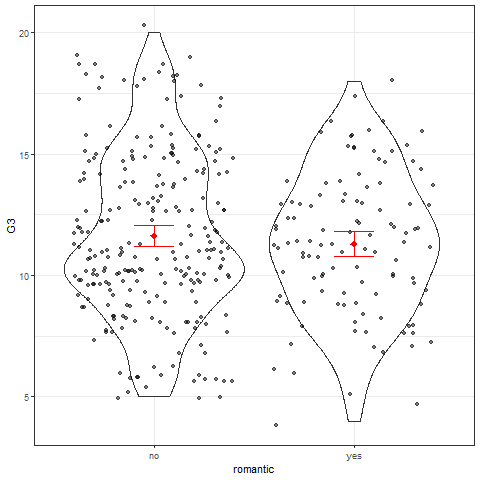
\includegraphics[width=6.67in]{../results/CI_plot}

\}

\textbackslash{}caption\{Figure 2: Mean and 95\% confidence interval for
final grades\}\label{fig:unnamed-chunk-5} \textbackslash{}end\{figure\}

In the single group, the estimate of the population parameter, the mean
of G3(final grade) is 11.63265. Here, we used boostrapping to come up
with a 95\% confidence interval for the estimate, {[}11.19582,
12.03265{]}. The emean of G3(final grade) falls within this 95\%
confidence interval.

In the in-relationship group, the estimate of the population parameter,
the mean of G3(final grade) is 11.28571. Here, we used boostrapping to
come up with a 95\% confidence interval for the estimate, {[}10.75871,
11.82143{]}. The mean of G3(final grade) falls within this 95\%
confidence interval.

\subsection{Hypothesis Testing and
Results}\label{hypothesis-testing-and-results}

To better explore the effect of having an romantic relationship, we
conduct a two sample Welch's t-test (
\href{https://en.wikipedia.org/wiki/Welch\%27s_t-test}{Reference}: two
samples have unequal variances and unequal sample sizes).

\textbf{Null hypothesis}: romantic relationship has no effect on final
grade

\textbf{Alternative hypothesis}: romantic relationshp will effect
student's final grade

\textbf{Significance level}: choose alpha = 0.05

\emph{Table 3. Results of the t-test}

\begin{longtable}[]{@{}rrrrrrrrrll@{}}
\toprule
X & estimate & estimate1 & estimate2 & statistic & p.value & parameter &
conf.low & conf.high & method & alternative\tabularnewline
\midrule
\endhead
1 & 0.3469388 & 11.63265 & 11.28571 & 0.9971016 & 0.319687 & 248.0219 &
-0.3383694 & 1.032247 & Welch Two Sample t-test &
two.sided\tabularnewline
\bottomrule
\end{longtable}

From the t-test, we have t-statistics = 0.9971016 and p-value =
0.319687. Since p-value \textgreater{} alpha = 0.05, we fail to reject
the null hypothesis that romantic relationship has no effect on final
grade.

\subsection{Limitations}\label{limitations}

\begin{enumerate}
\def\labelenumi{\arabic{enumi}.}
\item
  Limited sample: Although we have a total of 357 observations, the
  number of samples in the two groups are unevenly. Specifically, we
  have 245 in non-relationship group and only 112 in romantic
  relationship group. The relative small number (112) in one test group
  probably reduce the power of our test
\item
  Limited comparison scale: The final grade has a range of 0 to 20,
  while this is enough for a test on group means, the difference is
  certainly less pronounced than a grade scale of 0 to 100.
\item
  No control on other variables: Maybe those engaged in relationships
  all have significantly higher freetime than single students. So the
  added freetime canceled the negative effect of relationship. We don't
  know.
\end{enumerate}

\subsection{Future Directions}\label{future-directions}

\begin{enumerate}
\def\labelenumi{\arabic{enumi}.}
\tightlist
\item
  Increase sample size, especially for students in relationship groups
\item
  control on more variables, such as age, free-time, gender, etc.
\end{enumerate}

\subsection{External Sources}\label{external-sources}

\url{https://archive.ics.uci.edu/ml/datasets/Student+Performance}
\url{https://en.wikipedia.org/wiki/Welch\%27s_t-test}


\end{document}
